\newpage
\section{Hypermedia}



\subsection{Definition}
Die geläufigste Form von Hypermedia ist HTML in Verbindung mit dem Internet und Millionen von Websites. Hypermedia auf Websites zeichnet sich auf den ersten Blick durch zwei wesentliche Merkmale aus. Websites bestehen zum einen aus multimedialen Inhalten und sind zum anderen untereinander mit Verweisen verknüpft. Außerdem gibt es die Möglichkeit Daten an den Server über Formulare zu senden. Diese Merkmale lassen sich dem bekanntesten Hypermediaformat, (X)HTML ohne weiteres zuschreiben.\\
Roy Fielding beschreibt im Rahmen seiner Dissertation Representational State Transfer (REST)als einen Architekturstil, auf Grundlage des modernen Internets. Fielding definiert das Internet hierbei als ein hochgradig verteiltes Hypermedia-System, dessen Verteilung über die geographische Ausdehnung hinaus geht und eine grenzenlose Verbindung von Informationen ermöglicht. Dienstanbieter müssen mit einer unabhängigen Entwicklung von Software Komponenten sowie der unregulierten Skalierung des Internet zurecht kommen. Als Schlüsseltechnologie kommt an dieser Stelle Hypermedia zum Einsatz. Hypermedia ist im Rahmen des Internets ein einheitliches Mittel um auf Dienste zuzugreifen. Der Zugriff erfolgt über eingebettete Steuerelemente als ein Teil der erhaltenen Informationen.\tocite{fielding}{3}\\
Hypermedia bildet zudem eine universell einsetzbare Schnittstelle im Internet. Die gleiche Schnittstelle kann unabhängig von verschiedenen Informationsquellen genutzt werden. Verweise erlauben eine unbegrenzte Strukturierung der Informationen und die Manipulation der Verweise ermöglicht einem Dienstanbieter die Darstellung komplexer Beziehungen zwischen Informationen. Das Führen eines Dienstkonsumenten durch eine Anwendung ist auf diese Weise realisierbar. Außerdem können einfache Anfragen durchgeführt werden, die das Durchsehen von großen Datenbeständen vereinfachen. Einfachheit und Allgemeingültigkeit lassen Hypermedia zu einer leicht zugänglichen Technologie werden. \tocite{fielding}{67f}\\
REST abstrahiert von den implementativen Details, und fokussiert den Einsatz von Hypermedia mit der Interpretation von signifikanten Datenelementen durch selbst beschreibende Nachrichten. Diese  Hypermedianachrichten bestehen aus sechs Datenelementen:
\begin{itemize}
\item Ressource
\item Ressourcenidentifikator
\item Repräsentation der Information
\item Metadaten der Repräsentation
\item Metadaten der Ressource
\item Steuerdaten
\end{itemize}
Dinge der realen Welt werden durch die Ressource repräsentiert. Die Ressource selbst stellt eine Abstraktion der Information dar und kann einen Dienst, ein Dokument oder eine Sammlung anderen Ressourcen beinhalten.Der Ressourcenidentifikator dient der Adressierung und Referenzierung einer Ressource. Eine stabile und semantisch korrekte Identifikation liegt hierbei in der Verantwortung der Ressourcen verwaltenden Komponente. Die Repräsentation einer Ressource besteht aus Nutzdaten und Metadaten der Repräsentation zu Beschreibungszwecken. Zusätzlich kann eine Antwort auch Metadaten der Ressource enthalten. Diese beinhalten Informationen der Ressource, die nicht spezifisch zu der Repräsentation zugeordnet werden können. Die Steuerdaten dienen der Parametrisierung einer Anfrage. Sie beschreiben die Bedeutung und Verwendung einer bestimmten Aktion innerhalb der Nachricht.\tocite{fielding}{86ff}\\

"Hypermedia is defined by the presence of application control information embedded within, or as layer above, the presentation of information."\footnote{Fielding, 2000, S. 68}\\

Während des Entwurfs einer verteilten Hypermedia-Anwendung müssen diese Anforderungen durch den Einsatz eines bestimmten Datenformats abgebildet werden. Die Betrachtung von verschiedenen Hypermediaformaten soll innerhalb dieser Arbeit losgelöst von Programmiersprachen, Technologien und serverseitigen Implementationen erfolgen. Im Mittelpunkt steht eine Betrachtung der Formate entsprechend ihrer Eigenschaften und Fähigkeiten eine Hypermedia-Anwendung zu unterstützen.


\subsection{Richardsons Maturity Model}
Leonard Richardson beschreibt mit seinem Maturity Model eine Art Stufenplan, wie ein verteiltes Hypermedia System auf Basis von Internet Technologien umgesetzt werden kann. Die Konsequente Umsetzung von REST als Architekturstil und das Nutzen bestehender Technologien steht hierbei im Fokus. Das Zusammenwirken von HTTP, URIs und Hypermedia in Form von HTML ist charakteristisch für das Internet. Diese drei Technologien und dessen Kombination bilden die Grundlage für das erstellen einer Hypermedia Anwendung.\footnote{Richardson, L. (2008), \url{http://www.crummy.com/writing/speaking/2008-QCon/act3.html}}\\
\begin{center}
		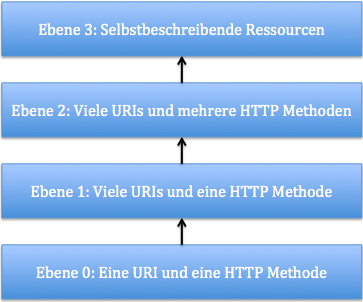
\includegraphics[width=8cm]{graphicx/maturity.png}
		\captionof{figure}{Leonard Richardsons Maturity Model}
		\label{hfaktoren}
	\end{center}
Um die Unterschiede zwischen den einzelnen Ebenen darzustellen wird ein sehr einfaches Warenwirtschaftssystem eingeführt. Dieses System bietet die Möglichkeit eine Liste des gesamten Warenbestands anzufragen, die Details einer bestimmten Ware anzuzeigen und Bestellungen von Waren auszulösen.\\
\begin{center}
		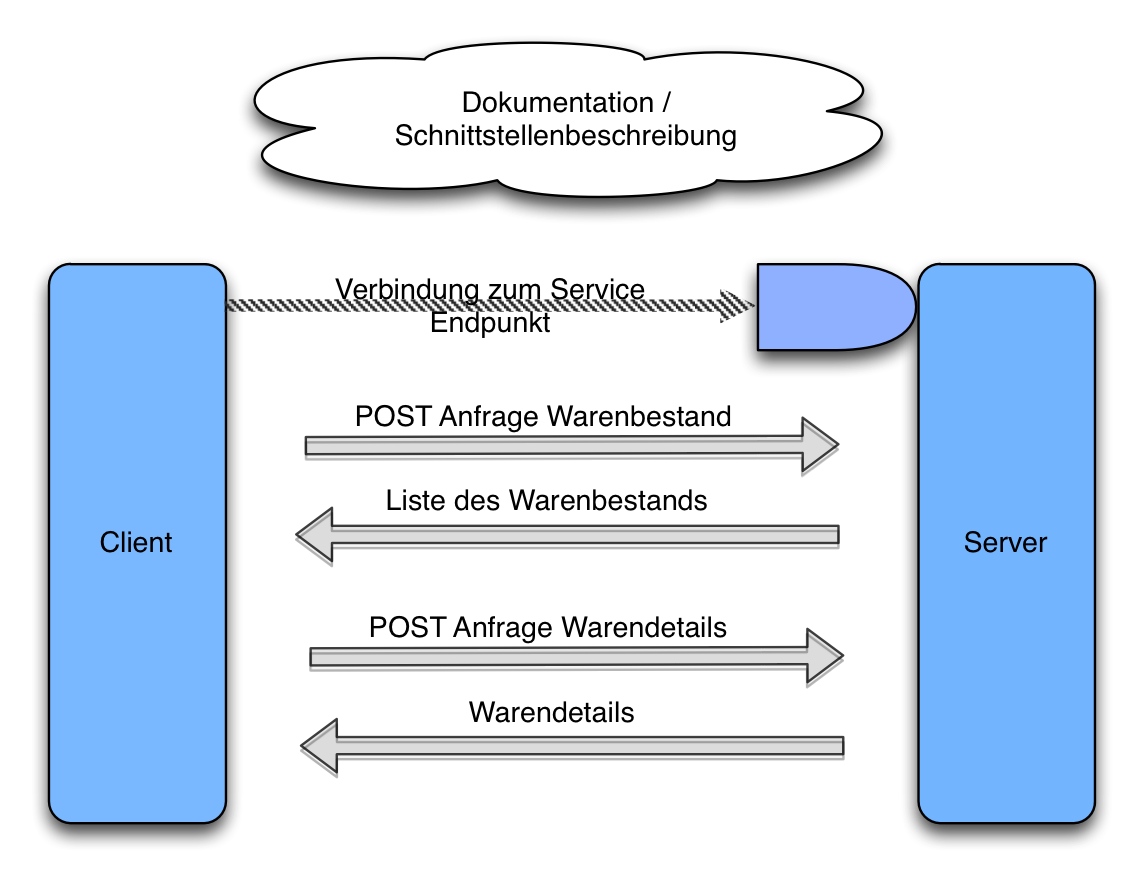
\includegraphics[width=10cm]{graphicx/MaturityLvL0.png}
		\captionof{figure}{Maturity Model Ebene 0}
		\label{hfaktoren}
	\end{center}
Auf Ebene 0 sind alle Funktionen außerhalb der Nachrichten definiert und werden in der Regel durch ein HTTP-POST getunnelt. HTTP dient auf dieser Ebene als Intermediär und löst selbst implementiere, entfernte Prozeduren oder Methoden aus. Diese Vorgehensweise ähnelt stark dem Konzept der Remote Method Invocation im Fall von JAVA. Die Kommunikation basiert auf dem serialisieren und deserialisieren von Objekten. Sämtliches Wissen über die Objekte und deren Format ist in einer externen Dokumentation festgelegt. Beispielhaft hierfür ist der Einsatz von "Plain old XML" (POX). Das Verständnis über die ausgetauschten XML-Instanzen liegt innerhalb einer Dokumentation und XML-Schemata werden zur Validation eingesetzt. Dies ist auch der Fall beim "Simple Object Access Protocol" (SOAP), der als ein industrieller Standard für den Austausch von Daten eingesetzt wird. Im Unterschied zu POX wird die XML-Instanz hier jedoch in eine Art Umschlag verpackt. Die Dokumentation erfolgt in einer Beschreibungssprache und liegt somit ebenfalls in externer Form vor.




\begin{center}
		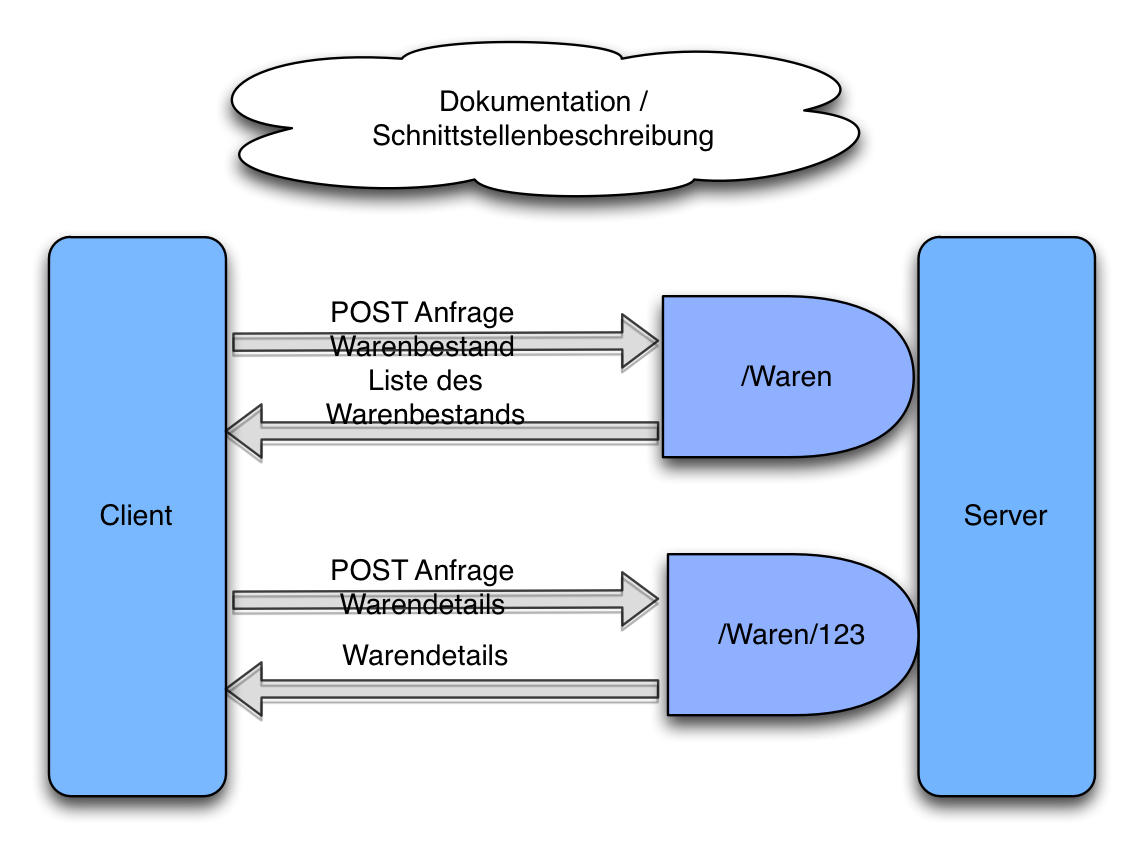
\includegraphics[width=10cm]{graphicx/MaturityLvL1.png}
		\captionof{figure}{Maturity Model Ebene 1}
		\label{hfaktoren}
	\end{center}
Die Verwendung von Ressourcen kommt auf Ebene 1 zum Tragen. Anstatt alle Anfragen an einen zentraler Endpunkt zu richten, werden auf dieser Ebene Ressourcen direkt angesprochen. Das Konzept der Ressourcen ermöglicht somit eine Art Identifikation von Dingen der Realen Welt. Sollten Details zu einer bestimmten Ware benötigt werden, kann diese nun direkt angesprochen werden. GET ist im Rahmen von HTTP definiert als eine sichere idempotente Operation, die keine signifikanten Änderungen am Status der Anwendung durchführt. Außerdem ist es möglich eine GET Anfrage, im Gegensatz zu einer POST Anfrage, zu cachen. Caching ist einer der wesentlichen Erfolgsfaktoren für eine performante Anwendung. Die Abfrage des Warenbestandes muss aufgrund ihres lesenden Charakters und der Beibehaltung des Anwendungszustands ab dieser Ebene mittels einer GET Anfrage durchgeführt werden. 




\begin{center}
		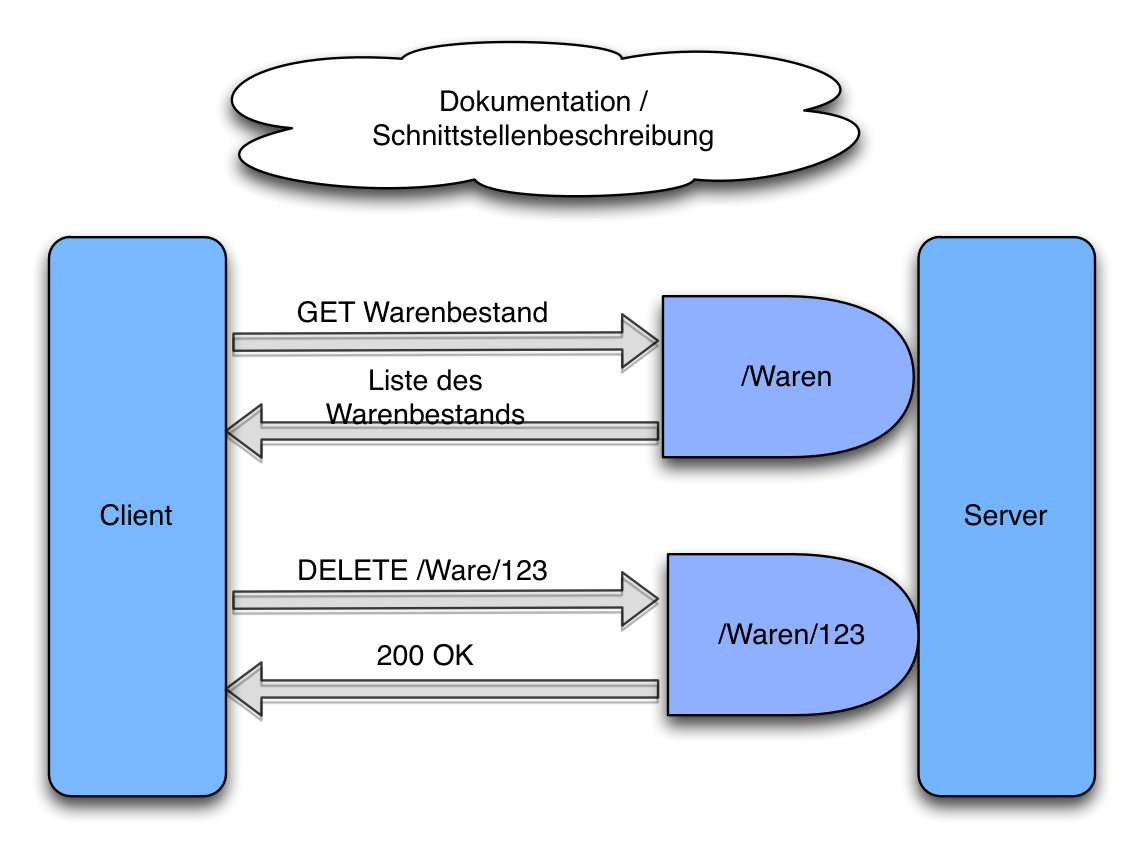
\includegraphics[width=10cm]{graphicx/MaturityLvL2.png}
		\captionof{figure}{Maturity Model Ebene 2}
		\label{hfaktoren}
	\end{center}
Eine Unterscheidung zwischen lesenden, schreibenden, idempotenten und nicht idempotenten Operationen konnte bis jetzt durch den Einsatz von HTTP als Tunnelmechanismus nicht vorgenommen werden. Eine entfernte Methode wurde stets durch ein POST ausgelöst. Die HTTP konforme Verwendung der Verben wird auf Ebene 2 eingeführt. Anstatt die Liste des Warenbestands über eine POST Anfrage auszuführen wird eine GET Anfrage abgesetzt. PUT, POST und DELETE sind im innerhalb von HTTP definiert als Operationen mit schreibendem Charakter und demzufolge einer Änderung des Anwendungszustands. Wenn eine Ware geändert oder gelöscht werden soll muss eine entsprechende Operation verwendet werden. Neben der korrekten Verwendung der Verben wird auf dieser Ebene ein Mechanismus zur Fehlerindikation eingesetzt. Die Verwendung der HTTP Status Codes entsprechend ihrer Spezifikation kann diese Rolle übernehmen. So muss zum Beispiel die korrekte Abarbeitung einer Anfrage vom Dienstanbieter mit einem "200 OK" quittiert werden. Die Umsetzung eines geeigneten Fehlerindikators liegt in der Verantwortung des Dienstanbieters.



\begin{center}
		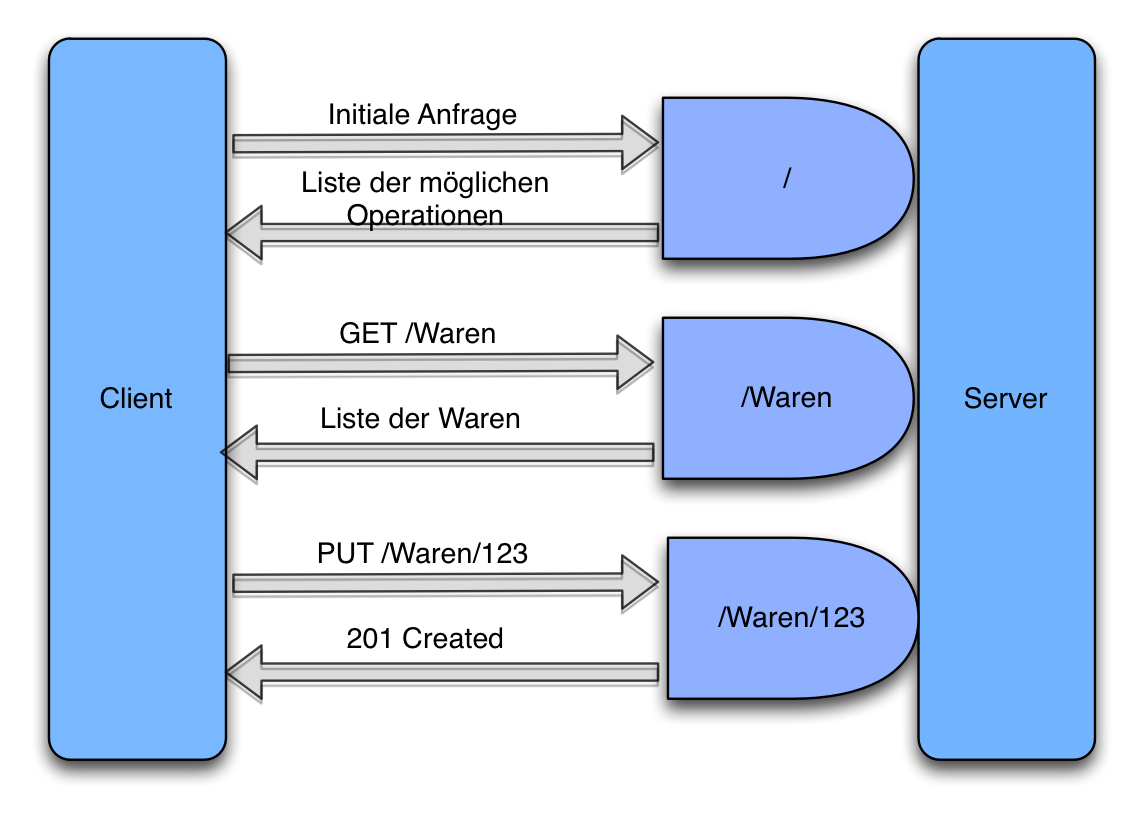
\includegraphics[width=10cm]{graphicx/MaturityLvL3.png}
		\captionof{figure}{Maturity Model Ebene 3}
		\label{hfaktoren}
	\end{center}
Ebene 3 beginnt mit der Verwendung von Hypermedia Steuerelementen. Eine Nachricht auf dieser Ebene enthält nicht nur reine Nutzdaten sonder auch semantische Informationen zum Verständnis der Daten. Hypermedia Steuerelemente zeigen einem Client welche Operationen er von seiner aktuellen Position aus durchführen kann. Der Client benötigt keine Kenntnis über die exakten Adressen für bestimmte Operationen. Vielmehr wird er vom einem zentralen Einstiegspunkt per Verweis den Anwendungsprozess geführt. Diese selbstbeschreibenden Nachrichten ermöglichen einen variablen Adressraum auf der Seite des Dienstanbieters und reduzieren die Kopplung zwischen Client und Server. Zudem kann der Dienstanbieter neue Verweise und Informationen zu seinen Nachrichten hinzufügen. Solange alle Dienstkonsumenten unbekannte Verweise ignorieren bietet der Einsatz von Hypermedia Steuerelementen eine gefahrlose Erweiterungsmöglichkeit der Nachrichten. Wenn das Warenwirtschaftssystem auf dieser Ebene operiert, benötigt der Client als Information nur den zentralen Einstiegspunkt und Kenntnis über die genutzten Verweise. Im Idealfall ist keine externe Dokumentation mehr nötig. Der Client kennt die benutzten Verweise und weiß anhand der selbstbeschreibenden Nachrichten mit welchen Operationen er auf eine Ressource zugreifen kann.\\
Das Richardson Maturity Model bietet keinen direkten Ansatz zur Bewertung eines bestimmten Hypermedia Formats. Es beschreibt jedoch Eigenschaften die für das Erstellen einer REST konformen Anwendung und damit einer Hypermedia Anwendung nötig sind. Besonders die Erfordernisse der dritten Ebene beschreiben Eigenschaften, die im Einflussbereich verschiedener Hypermedia Formate liegen. Eine detaillierte Betrachtung des eingesetzten Formats ist nötig um eine gute Anwendung zu erstellen und die gegebenen Vorteile im vollen Umfang zu nutzen. Dieser Anspruch impliziert die hohe Bedeutung für das Erstellen einer Vergleichsgrundlage für verschiedene Formate.









\subsection{Hypermedia Faktoren nach Amundsen}
Der Hypermediagedanke entstand aus der Fragestellung, wie man ein gutes verteiltes Informationssystem entwerfen kann. Grundsätzlich gibt es verschiedene Ansätze um ein verteiltes System zu entwerfen und die Komponenten miteinander kommunizieren zu lassen. Die zu gründe liegende Fragestellung ist hier, wie kann der Server private Objekte exportieren um sie für den Client sichtbar und benutzbar zu machen. Hierfür gibt es unterschiedliche Plattform- und sprachspezifische Lösungen. Die grundsätzliche Funktionsweise ist hierbei immer ähnlich. Die Objekte werden serialisiert über das Netzwerk geschickt und so an den Client zur Verarbeitung übergeben. Der Client selbst muss also über ein Verständnis der Daten verfügen. Diese Herangehensweise hat den Nachteil, dass eine Änderung der serialisiebaren Objekte auch eine Änderung des Clients zur Folge hat. Somit entsteht immer ein gewisser Grad an Kopplung zwischen Client und Server.\\

Amundsen beschreibt mit Hypermedia einen anderen Lösungsansatz. Eine Synchronisation von Client und Server, bei der private Datentypen miteinander geteilt werden ist nicht der richtige Ansatz. Stattdessen sollte eine Technik zur Datenbeschreibung unabhängig von Platform, Sprache und privaten Datentypen verwendet werden. Diese Herangehensweise nennt Amundsen die Hypermedia Lösung. Die Probleme des Typemarshalling werden im Fall von Hypermedia durch das Anreichern der Nachrichten mit zwei Arten von Metadaten gelöst. Ein Teil sind Metadaten über die Daten selbst. Der andere Teil sind Metadaten über den Applikationsstatus und die die Möglichkeiten für den Client, den Applikationsstatus zu ändern. Losgelöst von privaten Datentypen ermöglicht dieses nachrichtenorientierte Design, eine spezifischere Anpassung an die Anforderungen der Problemdomäne. Durch Hypermedia Nachrichten werden somit keine privaten Datentypen geteilt sondern vielmehr ein generelles Verständnis der Daten.\tocite{mamund}{10}\\
Nach Amundsen besteht eine Hypermedia Nachricht somit aus insgesamt drei Teilen:
\begin{itemize}
\item Daten
\item Metadaten über die Daten
\item Metadaten über den Applikationsstatus
\end{itemize}
Um Hypermedia selbst zu identifizieren, definiert Amundsen eine Sammlung abstrakter Eigenschaften und Funktionen, wie ein Hypermediaformat diese drei charakteristischen Datenteile umsetzt. Diese Sammlung wird Hypermediafaktoren (H-Faktoren) genannt und ist grundsätzlich unabhängig von der verwendeten Plattform und dem Transportprotokoll. In der Regel wird bei Hypermedia-Applikationen HTTP als Transportprotokoll eingesetzt, weil es eine Reihe von Vorteilen wie z.B. Nachhing, Chunking und Kompression bereits implementiert hat. HTTP ist aber keine zwingende Vorraussetzung für den Einsatz von Hypermedia. Diese H-Faktoren unterteilen sich dann noch in die zwei Bereiche Links und Control Data. Diese insgesamt neun H-Faktoren bilden das Gerüst für ein beliebiges Hypermediaformat. So kann man anhand dieser Faktoren bestimmet, ob ein bereits existierender Medientyp den Applikationsspezifischen Anforderungen genügt oder aber was bei der Erstellung eines eigenen Medientyps beachtet werden muss.\tocite{mamund}{13f}\\






Im Folgenden werden die einzelnen Faktoren genauer betrachtet. Die Link-Faktoren dienen im Wesentlichen der Bewegung des Clients im Applikationsfluss, wohingegen die Control Faktoren im dadurch definiert sind, dass sie zusätzliche Informationen beim Ausführen eines Verweises zur Verfügung stellen. Hier geht es vor allem um die Beschreibung der beinhalteten Nutzdaten. Die Berücksichtigung dieser Faktoren trägt dazu bei, dass alle Seiten etwas über die Beschaffenheit der Daten wissen oder aber die Daten in einer gewünschten Kodierung anzufordern. Die Illustration der H-Faktoren erfolgt am Beispiel von HTTP mit HTML als eingesetzten Hypermedia Typ. Die nachstehende Abbildung gibt einen Überblick der betrachteten Hypermedia Faktoren.\\
\begin{center}
		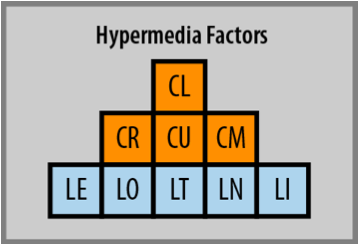
\includegraphics[width=8cm]{graphicx/hfaktoren.png}
		\captionof{figure}{Hypermedia Faktoren nach Amundsen}
		\label{hfaktoren}
	\end{center}



\subsubsection{Embedding Links}
Embedding Links(H-Faktor LE) dient der Darstellung einer Ressource im aktuell genutzten Ausgabefenster. Ein Embedding Link nutzt die Lesen-Operation des verwendeten Protokolls und stellt die Antwort innerhalb des aktuellen Fensters dar. Ein gebräuchliches Beispiel für Embedding Links sind auf einer Website eingebundene Elemente.\tocite{mamund}{15}\\
\begin{lstlisting}[caption={HTML Beispiel LE}\label{lst:code1},captionpos=t]
<iframe src="..."> Einbetten eines Rahmens
<img src="..."> Einbetten eines Bildes
\end{lstlisting}
Die im Listig 1 dargestellten Tags sorgen bei der Darstellung im Browser für eine Einbettung von lokalen oder entfernten Ressourcen und sind im Fall von HTML repräsentativ für den H-Faktor der Embedding Links.


\subsubsection{Outbound Links}
Outbound Links (H-Faktor LO) sind das, was man im Allgemeinen unter Navigationslinks versteht. Beim Folgen eines Outbound Links wird die Lesen-Operation des verwendeten Protokolls ausgeführt und die bestehende Ansicht durch die Antwort ersetzt.\tocite{mamund}{15} Die Antwort von Google auf eine Suchanfrage beinhaltet Outbound Links. Folgt man einem Verweis aus der Antwort wird die darauf folgende Antwort die aktuelle Ansicht ersetzen.\\
\begin{lstlisting}[caption={HTML Beispiel LO}\label{lst:code1},captionpos=t]
<a href="http://externe-domain.de">
\end{lstlisting}
In HTML werden Verweise durch das Anchor-Element (a) kenntlich gemacht. Die Kombination des Anchor- und Hyper-Reference- Elements ( a href) sorgt beim Aktivieren für eine Darstellung der refferenzierten Ressource in einer neuen Ansicht. 



\subsubsection{Templated Links}
Templated Links (H-Faktor LT) haben wie Embedding und Outbound Links nur einen lesenden Charakter. Templated Links ermöglichen dem Client das Senden von Daten an einen Server. Beispielsweise können bei einem Suchdienst die Parameter übergeben werden, so dass die Suchbegriffe als ein Teil des Links mit übermittelt werden. Die Zusammensetzung des Links ist abhängig von der Spezifikation des genutzten Medientyps. Ein Verweis der eine Suche durchführt, sollte entsprechend der Spezifikation wie im folgendem Listing zusammengesetzt sein.\tocite{mamund}{16}\\
\begin{lstlisting}[caption={HTML Beispiel LT}\label{lst:code1},captionpos=t]
<a href="http://externe-domain.de">
\end{lstlisting}
Templated Links für Suchanfragen in HTML bestehen nach Spezifikation aus der Zieldomain und einem Platzhalter für die vom Nutzer übergebene Zeichenkette.




\subsubsection{Idempotent Links}
Idempotent Links (H-Faktor LI) haben einen schreibenden Charakter und stellen eine Möglichkeit dar, Ressourcen auf dem Server anzulegen oder zu löschen. Idempotenz hängt hierbei natürlich von dem verwendeten Transportprotokoll und der serverseitigen Implementation ab. Bei der Verwendung von HTTP als Transportprotokoll sind GET,PUT und DELETE idempotente Operationen zur Kommunikation mit dem Server.\tocite{mamund}{16}\\
\begin{lstlisting}[caption={HTML Beispiel LI}\label{lst:code1},captionpos=t]
<form action="http://domain.de/ressource" method="put">
  <input type="submit"/>
</form>
\end{lstlisting}
Das im Listig dargestellte HTML-Formular dient dem Anlegen oder Aktualisieren einer Ressource. Durch das Method-Attribut ist festgelegt, welche Protokoloperation auf die Zielressource ausgeführt wird. Im Zusammenspiel von HTML und HTTP als genutztes Transportprotokoll ist PUT als eine idempotente Operation implementiert und führt auch bei mehrfacher Ausführung immer zum gleichen Ergebnis.


\subsubsection{Non-Idempotent Links}
Non-Idempotent Links (H-Faktor LN) bietet wie H-Faktor LI eine Möglichkeit Daten zu übertragen. Der Unterschied hier ist die Idempotenz. So liegt es in der Verantwortung des Medientyps zu definieren, wie mit nicht idempotenten Operationen umgegangen wird. Im Fall von HTTP ist die Methode POST als nicht idempotente Operation implementiert. POST wird genutzt um per Formular eine neue Ressource auf dem Server anzulegen.\tocite{mamund}{17}\\
\begin{lstlisting}[caption={HTML Beispiel LI}\label{lst:code1},captionpos=t]
<form action="http://domain.de/ressource" method="post">
  <input type="submit"/>
</form>
\end{lstlisting}
HTML-Formulare, die als Operation POST nutzen um Daten zum Server zu senden, legen eine neue Ressource auf dem Server an. Im Gegensatz zu PUT als idempotente Operation liefert POST nach der Durchführung nicht immer das gleiche Ergebnis. Stattdessen legt POST bei mehrfacher Ausführung, mehrere neue Ressource an. Der Umgang mit nicht idempotenten liegt in der Verantwortung und Implementation des konkret verwendeten Medientyps.





\subsubsection{Read Controls}
Read Controls (H-Faktor CR) beschreibt ob und wie die Möglichkeit besteht, eine lesende Operation zu reglementieren. Ein Beispiel hierfür sind die Accept-Header des HTTP Protokolls. Dem Client wird so die Möglichkeit gegeben ein bestimmtes Format oder die Antwort in einer bevorzugten Sprache anzufordern.\tocite{mamund}{18}\\
\begin{lstlisting}[caption={HTML Beispiel CR}\label{lst:code1},captionpos=t]
GET /beispiel/ressource HTTP/1.1
Host : domain.de
Accept : text/html
\end{lstlisting}
Read Control wird an dieser Stelle durch einen HTTP-Header veranschaulicht. Der Header resultiert aus einer lesenden Anfrage auf eine Ressource. Das Accept-Element im Header setzt hierbei die Steuerung der lesenden Operation GET um und schränkt die Annahme auf das Format HTML ein. Ressourcen mit mehreren Repräsentationsformen können auf diese Weise in einem spezifiziertem und vom Client unterstützen Format angefordert werden.


\subsubsection{Update Controls}
Update Controls (H-Faktor CU) bietet die gleichen reglementierenden Möglichkeiten, die der H-Faktor CR bietet für schreibende Operationen. Die Reglementierung von schreibenden Operationen kann bei HTTP z.B. durch das Content-Typ Feld im Header durchgeführt werden. So hat der Server Kenntnis darüber, in welcher Form ihm die Nutzdaten übergeben werden.\tocite{mamund}{18}\\
\begin{lstlisting}[caption={HTML Beispiel CU}\label{lst:code1},captionpos=t]
<form action="ressource/bild">
  <input type="file" accept="image/jpeg">
  <input type="submit">
</form>
\end{lstlisting}
Durch das Accept-Attribut wird der Upload einer Datei beschränkt. Das festlegen auf den Multipurpose Internet Mail Extension Type (MIME-Type) "image/jpeg" stellt sicher, dass eine neue Ressource, die über dieses Formular erstellt wird, den MIME-Type JPEG haben muss. Ein Anlegen von neuen Ressourcen kann somit exakt reglementiert werden. Elementarer Bestandteil der Reglementierung ist das Verwenden von MIME-Types. Eine Liste aller offiziell registrierten MIME-Types wird durch die Organisation "Internet Assigned Numbers Authority" (IANA) gepflegt und veröffentlicht.


\subsubsection{Method Controls}
Method Controls (H-Faktor CM) stellen Indikatoren dar, die beschreiben um was für eine Art von Operation es sich handelt bzw. welche Operation für einen konkreten Fall gültig sind. Ein HTML FORM-Element kann mit unterschiedlichen Methoden abgesendet werden. Das Attribut METHOD beschreibt an dieser Stelle mit welcher Operation des Transportprotokolls das Formular übertragen wird.\tocite{mamund}{18f}\\
\begin{lstlisting}[caption={HTML Beispiel CM}\label{lst:code1},captionpos=t]
<form action="ressource/bild" method="put">
<input type="submit"/>
</form>

<form action="ressource/bild" method="post">
<input type="submit"/>
</form>
\end{lstlisting}
Beide dargestellten Formulare senden ihre Nutzteten an "/ressource/bild". Sie unterscheiden sich jedoch in der verwendeten Protokolloperation. Durch die Method Controls kann am Beispiel von HTML festgelegt werden ob eine Ressource mit einer idempotenten oder mit einer nicht-idempotenten Operation angesprochen wird.



\subsubsection{Link Annotation Controls}
Zusätzlich zur Reglementierung von Schreib- und Leseoperationen kann ein Hypermedia Typ Link Annotation Controls (CL) unterstützen. Verweise werden dann mit semantischen Informationen angereichert. Clients, die diese Metadaten verstehen, können sich entsprechend der Semantik verhalten.
\begin{lstlisting}[caption={HTML Beispiel CL}\label{lst:code1},captionpos=t]
<div>
  <a href=".../seite1.html" rel="first">
  <a href=".../seite4.html" rel="next">
  <a href=".../seite2.html" rel="prev">
</div>
\end{lstlisting}
Dieses HTML Beispiel zeigt die Anreicherung der Links mit semantischen Informationen. Ein Client der die verwendeten Relationsattribute kennt kann die Sammlung von Verweisen durchsuchen und anschließend ohne seine eigene Position zu kennen auf die nächste, vorherige oder erste Seite navigieren. 



\subsubsection{Design Elemente}

Zusätzlich zu den 9 H-Faktoren definiert Amundsen vier Design-Elemente. Diese Design-Elemente stellen vor allem vier charakteristische Eigenschaften von Hypermedia Formaten dar. Aus diesem Grund werden sie im Folgenden beschrieben und im weiteren Verlauf zum Vergleich unterschiedlicher Formate verwendet.\\
Die vier Hypermedia Design-Elemente sind:\tocite{mamund}{20}
\begin{itemize}
\item Base Format
\item State Transfer
\item Domain Style
\item Application Flow
\end{itemize}

Jeder Hypermediatyp basiert auf einem bestimmten zugrundeligenden Format. Bekannte Formate sind XML, JSON, CSV und viele weitere. Ein Hypermediatyp kann auf einem beliebigen Basisformat aufbauen. Erst die Anreicherung des Basisformats mit zusätzlichen Metadaten und der Unterstützung von Hypermedia-Faktoren in einem bestimmten Umfang definieren einen Medientyp. Der Medientyp bestimmt außerdem ob eine Zustandsänderung der Applikation unterstützt wird oder nicht. Man kann hier unterscheiden zwischen der Art und Weise wie ein Zusatndsänderung durchgeführt werden kann. Hierbei gibt es drei Ausprägungen der Unterstützung. Keine Unterstützung bei nur lesenden Formaten. Definierte Unterstützung nach einer externen Dokumentation und Ad-Hoc Unterstützung mittels einer in die Nachricht eingebetteten Hypermedia Steuerung. Der Domain Style beschreibt wie stark ein Medientyp an eine Problemdomäne angepasst ist. Diese Stile sind kategorisiert als spezifisch, allgemein und agnostisch. Als letztes Design Element gilt es noch den Application Flow zu etwähnen. Hierbei geht es darum ob und in welchem Maße der Client in der Lage ist den Applikationsfluss zu steuern. Auch hier unterscheidet man drei Ausprägungen. Der Applikationsfluss kann entweder nicht, wesentlich oder hauptsächlich durch den Medientyp gesteuert werden.\tocite{mamund}{20}\\

\subsubsection{Hypermedia Ebenen}

Zusätzlich zu den Hypermedia-Faktoren und den Design Elementen definiert Amundsen noch vier Ebenen auf denen sich ein Hypermedia Typ befinden kann. Diese vier Ebenen sind aus der Sicht des Clients beschrieben und unterscheiden sich nach ihrem Möglichkeiten, in wie fern sie im Falle einer Veränderung angepasst werden müssen. Sie sind also gekennzeichnet durch einen bestimmten statischen und einen variablen Anteil. Statisch bezieht sich in diesem Kontext darauf, dass die statischen Anteile bei einer Veränderung oder Erweiterung der Applikation angepasst werden müssen. Die variablen Anteile hingegen können verändert werden ohne Probleme bei der Kommunikation zwischen Client und Server zu verursachen. Entweder dem statischen oder variablen Anteil zugeordnet werden die vier Eigenschaften Content, Address, Read Write Semantics und Appflow. Diese Eigenschaften sind wie folgt definiert:\footnote{Vgl. Amundsen, M. (2010), \url{http://amundsen.com/hypermedia/scraps/#hypermedia-levels}}
\begin{itemize}
\item Content beschreibt die Fähigkeit Elemente einer Nachricht hinzuzufügen oder zu entfernen.
\item Address ist definiert als die Möglichkeit, einen Unified Ressource Identidifier zu ändern, an den der Client seine Anfragen sendet.
\item Read Write Semantics ist eine Eigenschaft, bezüglich des Schreib-Leseverhaltens. Ein Hypermediatyp, der diese Eigenschaft besitzt ist in der Lage anzuzeigen, welche Elemente einer Nachricht schreibbar sind und welche Protokolfunktion zu benutzen sind.
\item Appflow bezeichnet die Möglichkeit den Applikationsfluss kontextbezogen zu steuern. Der Client benötigt nur die Antwort des Servers und kann die Steuerelemente der Nachricht benutzen um sich im Applikationsfluss zu bewegen.
\end{itemize}
Als Ebene 0 definiert Amundsen Serialisierte Objekte. Diese Ebene trifft auf Techniken wie SOAP und RPC-XML zu. Die Kommunikation zwischen Client und Server läuft über ein spezielles, Anwendungsbezogenes Nachrichtenformat. Die Definition der Kommunikationsregeln, also welches Format mit welchem Inhalt wo benutzt wird muss durch eine externe Dokumentation erfolgen. Diese Regeln werden dann im Client codiert und sie verfügen über keinerlei variablen Anteil. Die Konsequenz ist, dass der Client im Falle einer Änderung in allen vier Eigenschaften angepasst werden muss.\\

Ebene 1 ist beschrieben als standardisierte Datenformate. Beispielhafte Medientypen sind Comma Seperated Value (CSV) oder Extendible Markup Language (XML). Die Kommunikation zwischen Client und Server läuft über ein standardisiertes Datenformat. Dies hat den Vorteil, dass beide Seiten in der Lage sind den Nachrichten zu validieren. So können Elemente oder Attribute einer Nachricht hinzugefügt oder entfernt werden und die Kommunikation läuft weiterhin fehlerfrei. Der variable Anteil beschränkt sich jedoch auf die Eigenschaft Content. Die weiteren drei Eigenschaften sind nach wie vor statisch und eine Änderung würde zu Fehlern in der Kommunikation führen.\footnote{Vgl. Amundsen, M. (2010), \url{http://amundsen.com/hypermedia/scraps/#hypermedia-levels}}\\

Ebene 2 erweitert die standardisierten Datenformate mit Links. Atom und AtomPub sind Medientypen dieser Ebene. Der wesentliche Unterschied ist, dass ab dieser Ebene URIs in den Nachrichten enthalten sind. URIs werden somit nicht mehr im Client codiert sonder der Client bekommt mit jeder Nachricht URIs geliefert, denen er folgen kann. Dieser Fakt erweitert auch den variablen Anteil aus Ebene 1 um die Eigenschaft Address. Eine Anwendung, die einen Medientyp dieser Ebene benutzt kann ein variables URI-Schema benutzen. Sollte der Server seine URIs ändern, kann er dies tun ohne die Kommunikation zu bestehenden Client zu gefährden. Die Eigenschaften Read Write Semantics und Appflow sind weiter statisch.\footnote{Vgl. Amundsen, M. (2010), \url{http://amundsen.com/hypermedia/scraps/#hypermedia-levels}}\\

Ebene 3 ist genauso definiert wie Ebene 2, jedoch erweitert um die Möglichkeit der Applikationssteuerung. Die Kopplung zwischen Client und Server, die einen Medientyp dieser Ebene benutzen, besteht aus einer Vereinbarung über den verwendeten Datentyp und den Elementen einer Nachricht, die zur Applikationssteuerung benutzt werden. Der Client muss in der Lage sein die Steuerelemente einer Nachricht zu erkennen und dem Benutzer so die derzeit aktuellen Steueroptionen anzuzeigen. Hypermediaformate dieser Ebene sind unter anderem die Hypertext Markup Language (HTML) und VoiceXML.\footnote{Vgl. Amundsen, M. (2010), \url{http://amundsen.com/hypermedia/scraps/#hypermedia-levels}}\\

Betrachtet man die H-Level nach Amundsen etwas abstrakter, sind die Ebenen nach dem Grad der Kopplung zwischen Client und Server definiert. Wobei der Grad an Kopplung als Wissen verstanden werden kann, welches der Client über die Nachrichten haben muss. Dieses Wissen wird auch als "Out of Band Knowledge" bezeichnet. Der Verzicht, dieses Wissen innerhalb des Clients zu codieren, sorgt für eine bessere Flexibilität und Wartbarkeit des Gesamtsystems. Hypermediaformate ab der dritten Ebene betten ihre Nachrichten in einen semantischen Kontext. Die Kopplung besteht hier dann ausschließlich aus den definierten Steuerelementen und der Einigung über das Datenformat. Innerhalb dieser Arbeit werden die H-Faktoren und die vier Design-Elemente als Grundlage verwendet, um verschiedene Formate untereinander vergleichbar zu machen. Diese Ansicht ist nur als Vergleich zu sehen, da Hypermedia Typen nicht zwangsläufig alle H-Faktoren und Design Elemente unterstützen müssen. So kann ein rein zum lesen ausgelegter Medientyp z.B. auf das Design Element des Applikationsflusses verzichten. Ein gängiges Beispiel hierfür ist ein Atom-Feed Reader. Der Medientyp beinhaltet nur eine kurze Vorschau und einen Link auf den gesamten Artikel. Funktionen, die den Applikationsfluss steuern sind nicht notwendig.













\subsection{Design-Prozess}


\subsection{Anwendungsbeispiel}
